\documentclass[10pt,conference]{IEEEtran}
\IEEEoverridecommandlockouts

\usepackage{cite}
\usepackage{amsmath,amssymb,amsfonts}
\usepackage{algorithmic}
\usepackage{graphicx}
\usepackage{textcomp}
\usepackage{xcolor}
\usepackage{listings}
\usepackage{subcaption}
\usepackage{multirow}
\usepackage{url}
\usepackage{stmaryrd}
\usepackage{colortbl}
\usepackage{ctable}
\usepackage{makecell}
\usepackage{graphics}
\usepackage{float}

\lstset{basicstyle=\ttfamily}
\newcommand{\stextsf}[1]{\textsf{\small #1}}
\newcommand{\bigtool}{\textsf{JSTAR}}
\newcommand{\tool}{\stextsf{JSTAR}}
\newcommand{\jiset}{\stextsf{JISET}}

\lstdefinestyle{code}{
  numbers=none,
  extendedchars=true,
  basicstyle=\small\ttfamily,
  showstringspaces=false,
  showspaces=false,
  xleftmargin=\parindent,
  tabsize=2,
  breaklines=true,
  showtabs=false,
  captionpos=b
}

\newcommand{\code}[1]{\text{\lstinline[style=code]!#1!}}

\begin{document}

\title{$\bigtool$: JavaScript Specification Type Analyzer using Refinement}

\author{
  \IEEEauthorblockN{Jihyeok Park}
  \IEEEauthorblockA{\textit{School of Computing}\\
  \textit{KAIST}\\
  Daejeon, South Korea\\
  jhpark0223@kaist.ac.kr}

  \and

  \IEEEauthorblockN{Seungmin An}
  \IEEEauthorblockA{\textit{School of Computing}\\
  \textit{KAIST}\\
  Daejeon, South Korea\\
  h2oche@kaist.ac.kr}

  \and

  \IEEEauthorblockN{Wonho Shin}
  \IEEEauthorblockA{\textit{School of Computing}\\
  \textit{KAIST}\\
  Daejeon, South Korea\\
  new170527@kaist.ac.kr}

  \and

  \IEEEauthorblockN{Yusung Sim}
  \IEEEauthorblockA{\textit{School of Computing}\\
  \textit{KAIST}\\
  Daejeon, South Korea\\
  yusungsim@kaist.ac.kr}

  \and

  \IEEEauthorblockN{Sukyoung Ryu}
  \IEEEauthorblockA{\textit{School of Computing}\\
  \textit{KAIST}\\
  Daejeon, South Korea\\
  sryu.cs@kaist.ac.kr}
}

\maketitle

\begin{abstract}
  This document describes the artifact package accompanying the ASE 2021 paper
  ``$\tool$: JavaScript Specification Type Analyzer using Refinement.'' The
  artifact includes $\tool$ source code, the accepted paper, a companion report,
  ECMAScript (JavaScript specification) open-source repository as a git
  submodule, and scripts to replicate the data presented in the paper. $\tool$
  performs type analysis on any commit version of ECMAScript to detect
  type-related specification bugs. $\tool$ is an extended tool of $\jiset$, a
  JavaScript IR-based Semantics Extraction Toolchain. We hope that the artifact
  will be useful for contributors who update JavaScript specifications by
  automatically detecting type-related specification bugs before releasing them.
\end{abstract}

\begin{IEEEkeywords}
JavaScript, mechanized specification, type analysis, refinement, bug detection
\end{IEEEkeywords}

\section{Getting Started Guide}
The artifact is open-source can be obtained by cloning the following git
repository:
\begin{lstlisting}
$ git clone --recurse-submodules \
  https://github.com/kaist-plrg/jstar.git
\end{lstlisting}
Please see \code{INSTALL.md} for the detailed guide of installation, how to use
this artifact.  We also provide this artifact in Zenodo with a
DOI\footnote{https://doi.org/10.5281/zenodo.5084816} and docker image as
follows:
\begin{lstlisting}
$ docker run -it --rm jhnaldo/jstar
\end{lstlisting}

\section{Overall Structure}

\begin{figure}[H]
  \centering
  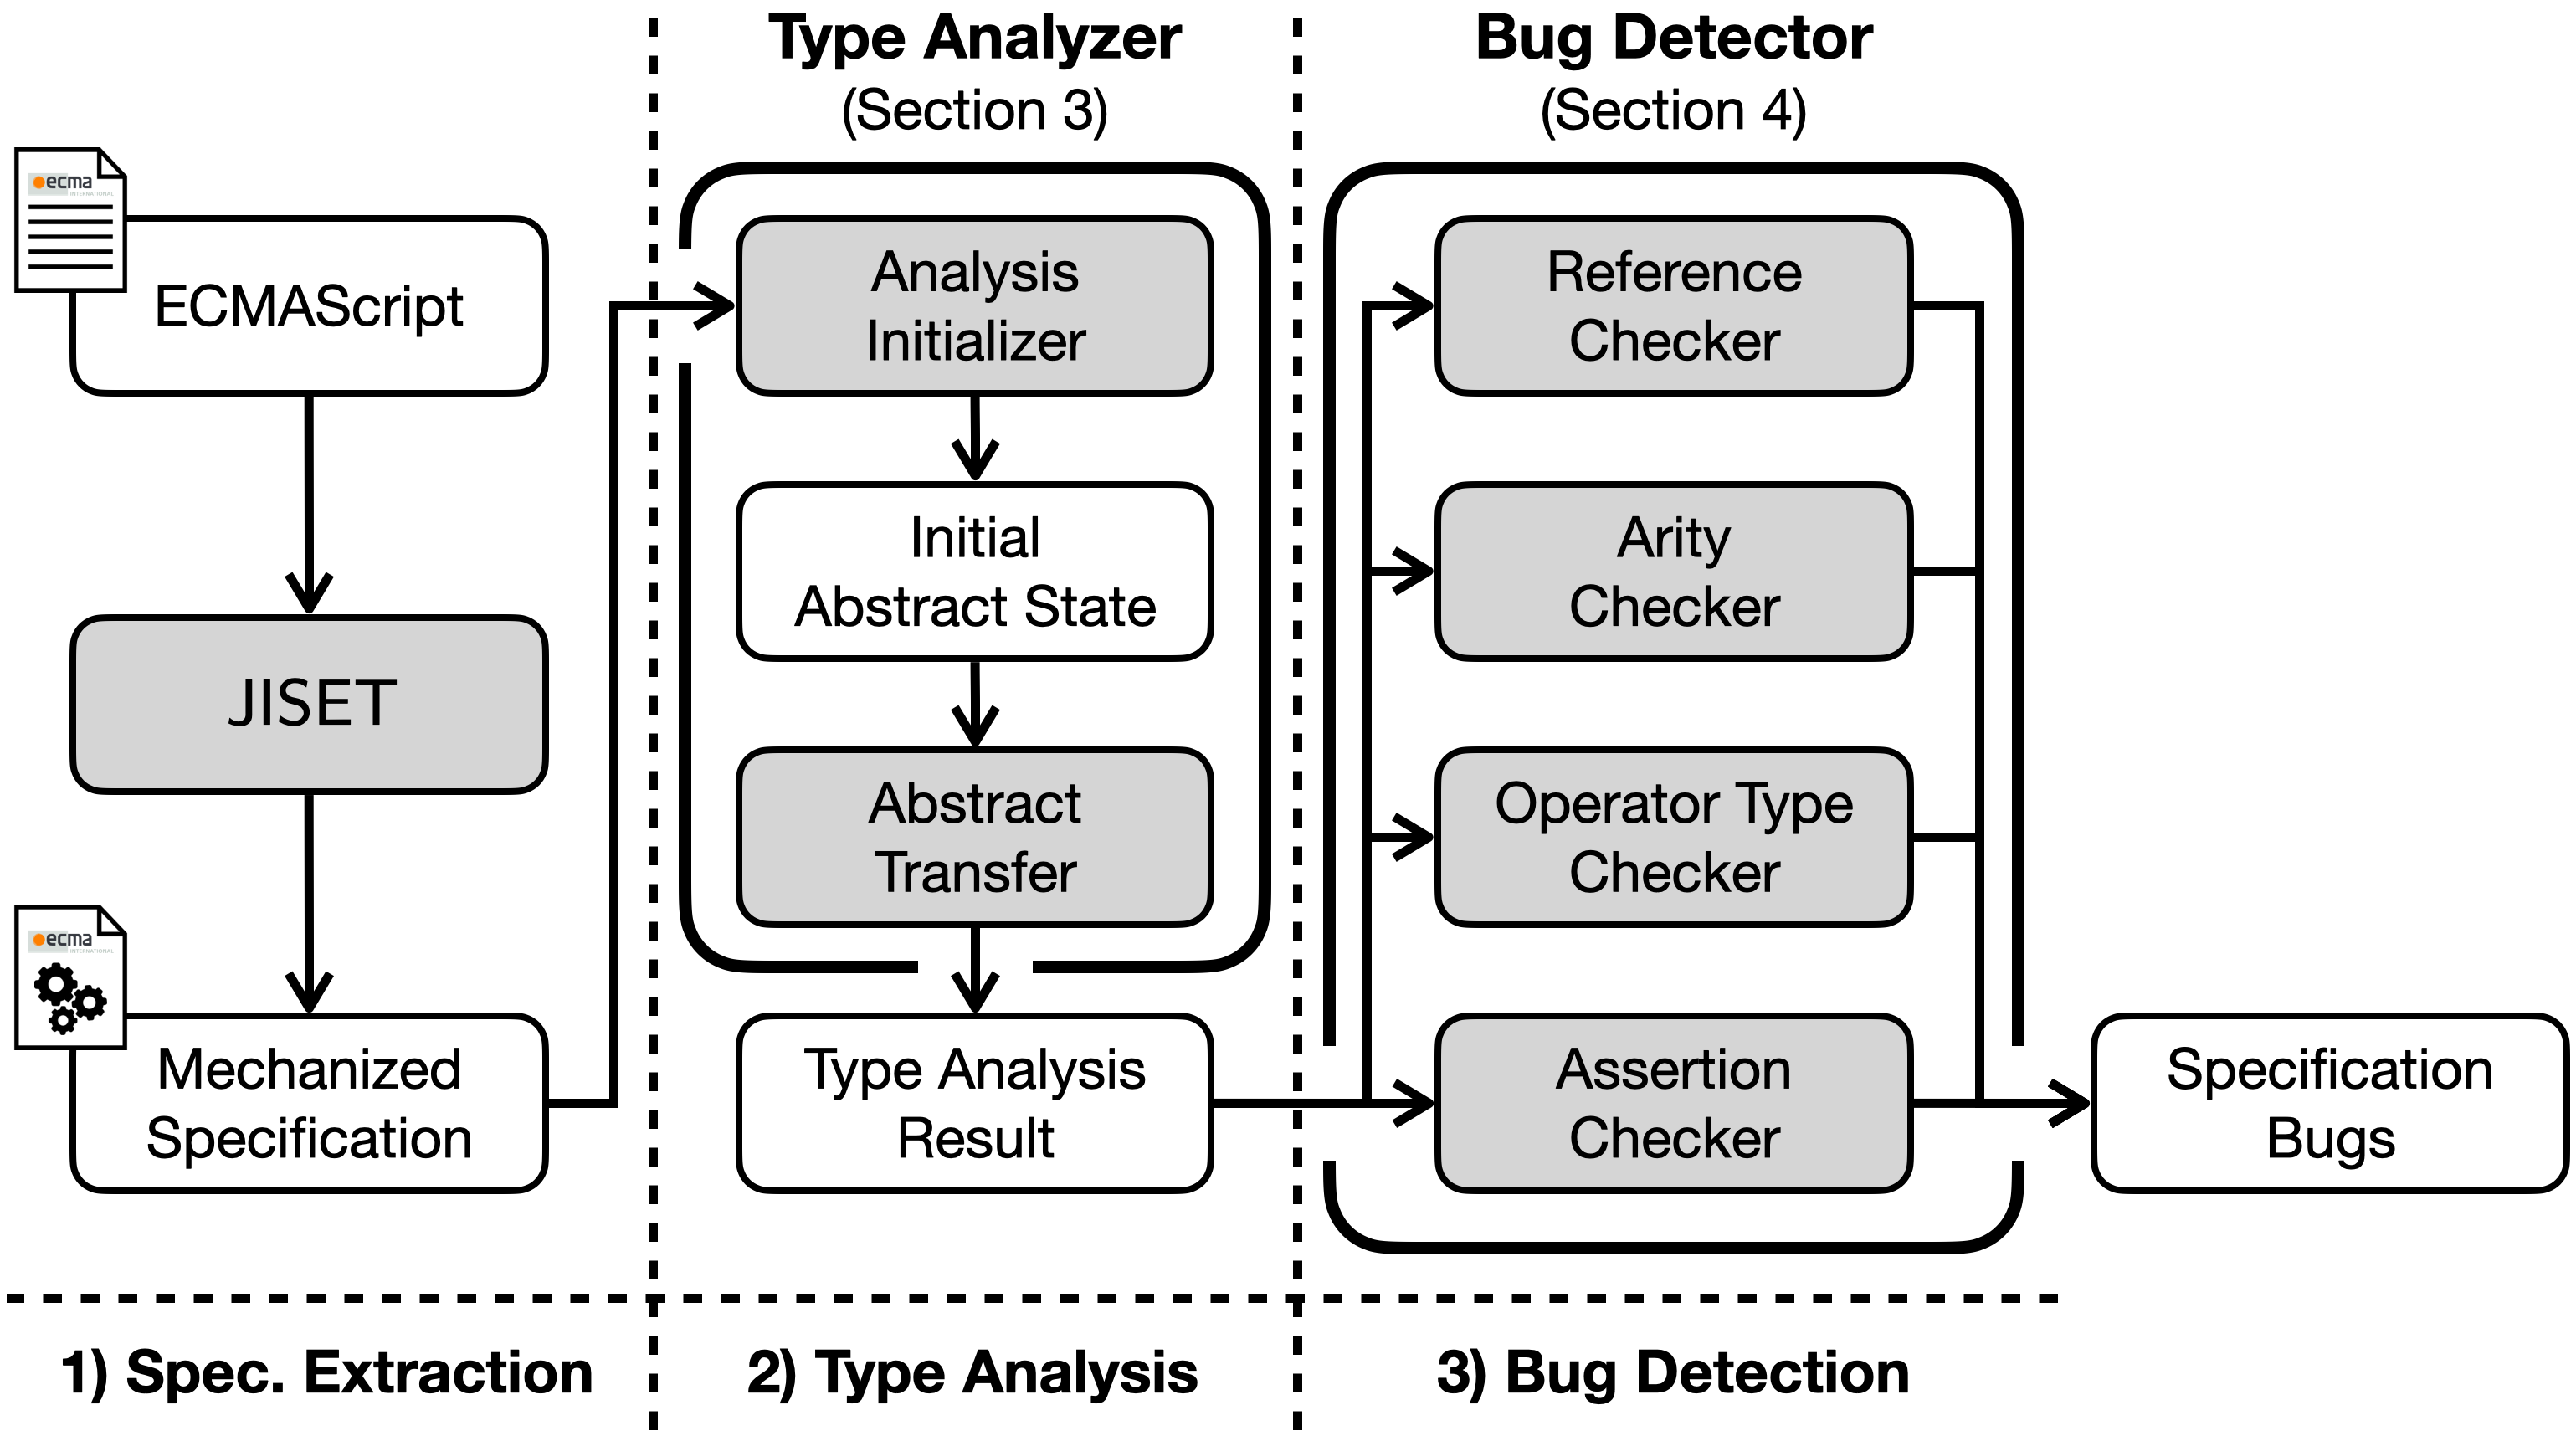
\includegraphics[width=\columnwidth]{../img/overall}
  \vspace*{-1.5em}
\end{figure}

$\tool$ consists of three phases: 1) specification extraction, 2) type analysis,
and 3) bug detection.  Details of the JSTAR framework are available in the paper
\code{ase21-park-jstar.pdf} and the companion report
\code{ase21-park-jstar-report.pdf}.

\subsection{Specification Extraction}
We utilizes another tool $\jiset$\footnote{https://github.com/kaist-plrg/jiset},
which is a \textbf{J}avaScript \textbf{I}R-based \textbf{S}emantics
\textbf{E}xtraction \textbf{T}oolchain, to extract a mechanized specification
from given ECMAScript.

\subsection{Type Analysis}
JSTAR performs a type analysis with flow-sensitivity and type-sensitivity for
arguments.  Each function is split into multiple flow- and type-sensitive views,
and an abstract state stores mapping from views to corresponding abstract
environments.  The type analyzer consists of two sub-modules: an
\textbf{Analysis Initializer} and an \textbf{Abstract Transfer Function}.
\begin{itemize}
  \item \textbf{Analysis Initializer} defines the initial abstract state and the initial
    set of views for a worklist.
  \item \textbf{Abstract Transfer Function} gets a specific view from the worklist and
    updates the abstract environments of the next views based on the abstract
    semantics for each iteration.
\end{itemize}

\subsection{Bug Detection}
To detect type-related specification bugs utilizing the type analysis, we
developed four checkers in a bug detector:

\begin{itemize}
  \item \textbf{Reference Checker} detects \textit{reference bugs} which occur
    when trying to access variables not yet defined (`UnknownVar`) or to
    redefine variables already defined (`DuplicatedVar`).
  \item \textbf{Arity Checker} detects \textit{arity bugs}. An arity bug occurs
    when the number of arguments does not match with the function arity
    (`MissingParam`).
  \item \textbf{Assertion Checker} detects \textit{assertion failures}. An
    assertion failure (`Assertion`) occurs when the condition of an assertion
    instruction is not true.
  \item \textbf{Operand Checker} detects \textit{ill-typed operand bugs}. An
    ill-typed operand bug occurs when the type of an operand does not conform to
    its corresponding parameter type.
\end{itemize}

\end{document}
